\chapter{Introduction} \label{chapitre-1}

Les concepts sur lesquels porte le travail décrit dans ce manuscrit sont définis dans cette première partie introductive. Tout d'abord, la technique du \gls{nfb}, 
qui est au centre de ce travail, est présentée, puis ses diverses applications sont listées. Dans la suite du manuscrit, seule l'une d'entre est étudiée : 
il s'agit du \gls{tdah} chez l'enfant, dont les principales caractéristiques sont exposées dans cette partie. 

Une fois le décor planté, les objectifs de cette thèse sont énoncés et la contribution de chaque chapitre est mise en évidence. Enfin, les analyses présentées 
ici ont fait l'objet de publications scientifiques et d'une communication orale dont les références sont fournies en fin de partie.  

\section{Définition du Neurofeedback}

Le \gls{nfb} est une technique d’apprentissage à visée thérapeutique permettant de modifier un paramètre d’activité cérébrale au moyen d’une 
information en temps réel associée à une récompense \citep{Arns2014}. 
La découverte et l'évolution de cette méthode sont retracées ici, puis son principe est décrit précisément.

\subsection{Historique}

Les prémices du \gls{nfb} remontent au début des années 1930, peu après l'enregistrement du premier \gls{eeg} humain par Hans Berger en 1929 \citep{Berger1929}.
En effet, \citet{Durup1935} et \citet{Loomis1936} ont observé que les ondes alpha, oscillant entre 8 et 12Hz, pouvaient être contrôlées grâce au 
conditionnement classique. 

Plus tard, ce qui peut être considéré comme le premier entrainement par \gls{nfb} a été mené par le Dr. Kamiya qui a demandé aux sujets de son étude 
de contrôler le rythme alpha et qui a obtenu des résultats prometteurs \citep{Kamiya1969}. 

Une preuve solide de la modulation de l'\gls{eeg} a été rapportée dans les années 1960 par le Dr. Sterman : l'expérience 
originelle consistait à entrainer le cerveau des chats en leur apprenant quoi faire pour obtenir de 
la nourriture. Durant cette expérience, le Dr. Sterman a extrait un rythme particulier au niveau du cortex sensorimoteur : le \gls{smr}, qui correspond 
aux fréquences entre 12 et 15Hz. Ensuite, le but du Dr. Sterman a été d'entrainer les chats à produire ce rythme en leur donnant de la nourriture 
lorsqu'ils réussissaient à l'émettre pendant une demi seconde, ce que les chats ont vite appris à faire. 

Cette modulation a ensuite été employée à des fins cliniques : l'entrainement du \gls{smr} chez les chats améliore leur sommeil \citep{Sterman1970} mais aussi
réduit la fréquence de leurs crises d'épilepsie après une exposition au kérosène \citep{Sterman1974}. 

Cependant, le \gls{nfb} ne correspondant pas à ce qui 
était connu à l'époque quant au fonctionnement du cerveau humain, son utilisation s'est faite en marge de la communauté scientifique \citep{Masterpasqua2003}. 
Il faut attendre les années 2000 pour que le \gls{nfb} soit réhabilité conduisant à une explosion du nombre d'études scientifiques visant à mieux comprendre 
ses mécanismes et ses effets, illustrée à la Figure~\ref{Figure:introduction_number_of_nfb_publications}. 

\begin{figure}[h!]
  \centering
	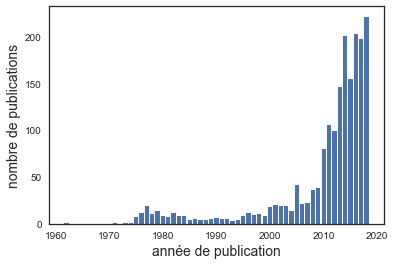
\includegraphics[width=0.7\linewidth]{figures/chapter-1/introduction-number-of-nfb-publications} 
  \caption{Evolution du nombre de publications sur le \gls{nfb} par année, entre 1962 et 2018. La base de données PubMed a été questionnée avec les 
	termes de recherche "Neurofeedback OR EEG Biofeedback".}
  \label{Figure:introduction_number_of_nfb_publications}
\end{figure}

\subsection{Principe du Neurofeedback}

Le \gls{nfb} a pour but d'apprendre à un sujet à auto-réguler son activité cérébrale à l'aide de retours auditifs et/ou visuels en temps réel
intégrés dans un jeu sérieux \citep{Wang2010}. Ces retours lui permettent de suivre la régulation de son rythme cérébral : si elle est modulée de 
la manière souhaitée, une récompense auditive et/ou visuelle est attribuée, sinon le sujet doit prendre une action corrective. Le \gls{nfb} 
est basé sur le conditionnement opérant \citep{Reynolds1975} : celui-ci se distingue du conditionnement classique où un stimulus conduit à 
une réaction automatique. En effet, dans le cas du conditionnement opérant, le conditionnement n'est pas lié à des réponses réflexes de
l'organisme mais à l'influence de l'environnement, qui renforce positivement ou négativement le conditionnement \citep{Skinner1948}. 

L'activité cérébrale enregistrée lors du \gls{nfb} est couramment l'\gls{eeg}, cependant d'autres modalités telles que l'imagerie par résonance 
magnétique fonctionnelle (\gls{fmri} en anglais) \citep{Sulzer2013} ou le couplage entre l'\gls{eeg} et la \gls{fmri} \citep{Perronnet2017} existent ; ici,
seul le \gls{nfb} \gls{eeg} est étudié. L'\gls{eeg} est enregistré de façon non-invasive au moyen d'électrodes placées sur le scalp, 
le bon contact entre la peau et les électrodes est représenté par une faible impédance, qui signifie que le niveau de bruit dans le 
signal est réduit \citep{Kappenman2010}. Le choix du nombre et du placement des électrodes se fait en fonction de l'application du \gls{nfb}, comme détaillé en 
\ref{applications_NFB}. Le signal passe ensuite par un amplificateur, qui peut être conforme à la norme ISO-60601-2-26 \citep{ISO}, avant d'être analysé 
par l'application de \gls{nfb}. 

Cette application extrait alors le marqueur à moduler, appelé par la suite neuromarqueur : celui-ci, tout comme les électrodes utilisées, 
dépend de l'application du \gls{nfb}. Le neuromarqueur correspond le plus souvent à des ondes cérébrales, isolées au niveau de certaines électrodes,
qui sont définies sur un intervalle de fréquence donné, qui peut varier selon les études \citep{Marzbani2016} :
\renewcommand{\labelitemi}{$\bullet$}
\renewcommand{\labelitemii}{$\cdot$}
\begin{itemize}
\item les ondes delta (moins de 4Hz),
\item les ondes theta (4-8Hz),
\item les ondes alpha (8-12Hz),
\item les ondes beta (12-30Hz), dont les ondes \gls{smr} entre 12 et 15Hz,
\item les ondes gamma (30-100Hz)
\end{itemize}
Pour certaines applications, le neuromarqueur est un ratio de deux ondes cérébrales \citep{Gevensleben2009}.

Le seuil auquel est comparé le neuromarqueur pour octroyer les récompenses visuelles et/ou auditives peut être fixe 
au cours de la session et/ou du traitement, ou alors incrémental intra ou inter-sessions. Par ailleurs, sa valeur, dans 
les deux cas, peut être définie soit par un praticien, soit être calculée automatiquement \citep{Arns2014}. La répétition de cet exercice mène au phénomène de 
neuroplasticité \citep{VanDoren2017, Ros2010} qui permet une réorganisation neuronale durable.

Toutes ces étapes sont résumées à la Figure~\ref{Figure:introduction_nfb_explications}.

\begin{figure}[h!]
  \centering
	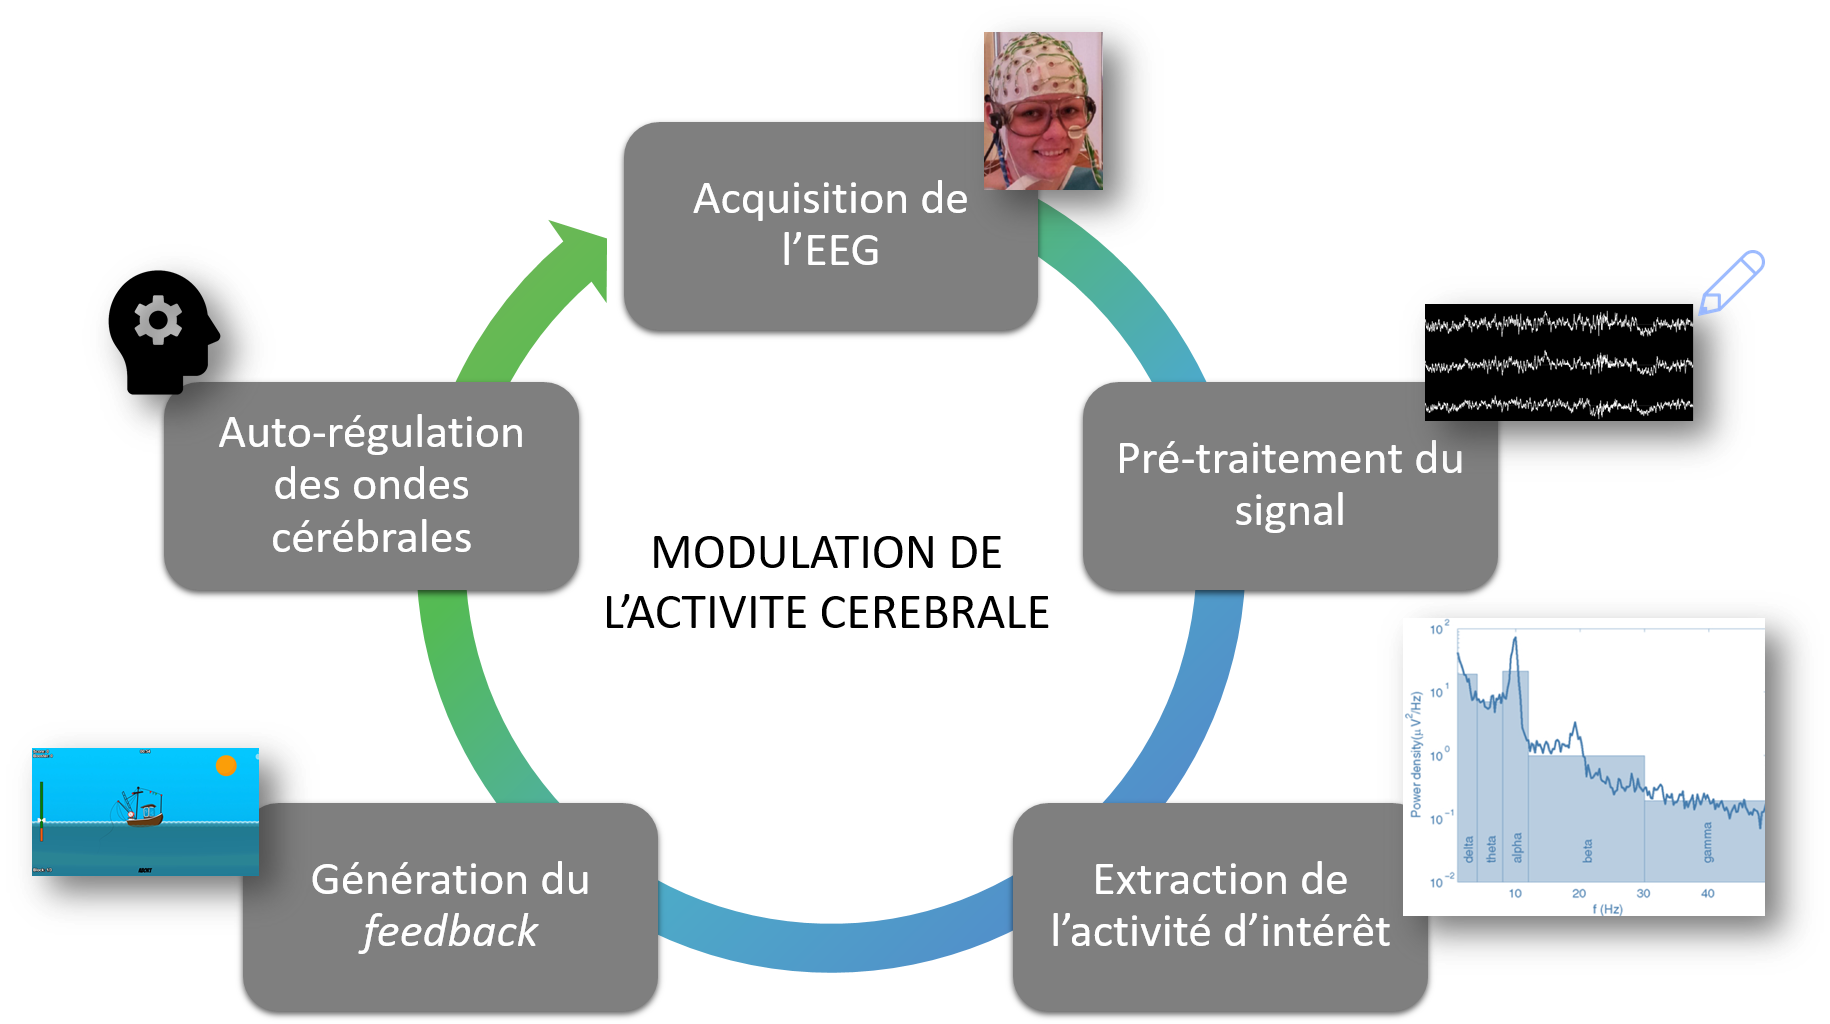
\includegraphics[width=1\linewidth]{figures/chapter-1/introduction-nfb-explication} 
  \caption{Schématisation du principe de \gls{nfb}.}
  \label{Figure:introduction_nfb_explications}
\end{figure}

Certaines applications de \gls{nfb} se démarquent des autres en proposant une correction ou un rejet des artefacts en temps réel des signaux \gls{eeg}
\citep{Maurizio2014, Barthelemy2019, Barthelemy2017} pour s'assurer que les récompenses sont bien calculées à partir du signal \gls{eeg} et non sur du bruit. 
Dans le cas où des artefacts sont détectés, l'utilisateur peut en être informé et adopter une action corrective, à l'instar de ce qui est implémenté dans 
\citep{Bioulac2019}

Quelquefois, une phase de transfert entre les blocs d'entrainement est intégrée. En effet, une session de \gls{nfb} est 
généralement sectionnée en blocs d'entrainement de quelques minutes, séparés par une courte période de repos. Entre ces blocs, certaines applications insèrent 
un bloc dit de transfert durant lequel aucun retour n'est donné à l'utilisateur alors que celui-ci doit moduler son activité cérébrale \citep{Bioulac2019,
Bluschke2016}. Cette phase de transfert a pour but de faciliter la transposition du contrôle appris durant les 
sessions de \gls{nfb} à la vie de tous les jours \citep{Arns2014}. Dans certains cas, afin d'aider à cette transposition, une carte représentant l'interface du jeu sérieux est 
fournie au sujet afin qu'il puisse la regarder en modulant son activité cérébrale en dehors des sessions de \gls{nfb} \citep{Leins2007}. 

Une autre différence que peuvent présenter les applications de \gls{nfb} est la personnalisation du \gls{nfb} selon le profil \gls{eeg} du sujet
\citep{Alkoby2017}. En effet, certaines applications proposent d'adapter les définitions des bandes de fréquences au sujet en utilisant la fréquence de son
pic alpha (\gls{iapf} en anglais) \citep{Alkoby2017, Escolano2014, Bazanova2018}, dont un exemple est présenté à la Figure~\ref{Figure:introduction_iapf}, 
qui est variable entre les sujets \citep{Haegens2014, Aurlien2004, Smit2006}. Par ailleurs, certaines applications de \gls{nfb} proposent d'entrainer 
le neuromarqueur qui correspond le mieux au profil \gls{eeg} du sujet \citep{Bioulac2019, Kerson2013}. 

\begin{figure}[h!]
  \centering
	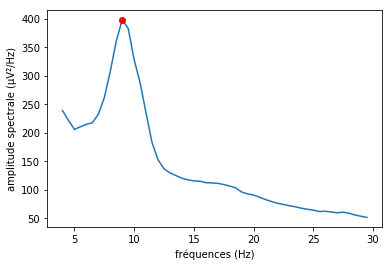
\includegraphics[width=0.5\linewidth]{figures/chapter-1/introduction-iapf} 
  \caption{Spectre d'un signal \gls{eeg} obtenu les yeux fermés au repos. L'\gls{iapf} correspond au point rouge.}
  \label{Figure:introduction_iapf}
\end{figure}

\section{Les champs d'application du Neurofeedback} \label{applications_NFB}

Le \gls{nfb} présente de nombreuses applications dont les principales sont détaillées ici. Parmi ces applications, l'une d'entre elles est présentée 
plus précisément car elle est exclusivement étudiée dans la suite : le \gls{tdah} chez l'enfant.

\subsection{De nombreuses applications}

Comme détaillé précédemment, l'\gls{eeg} comporte plusieurs composantes fréquentielles dont chacune correspond à une fonction physiologique différente.
En effet, par exemple, les ondes delta sont observées lorsque le sujet est endormi, les ondes theta lorsqu'il somnole, les ondes alpha lorsqu'il est relaxé, 
les ondes beta lorsqu'il est attentif et les ondes gamma lorsqu'il est en plein processus cognitif \citep{Marzbani2016}. 

Par ailleurs, afin d'interpréter la présence de ces ondes sur l'\gls{eeg}, il faut prendre en considération les électrodes sur lesquelles elles sont observées 
car chaque aire cérébrale a des fonctions spécifiques, comme par exemple \citep{Marzbani2016} :
\begin{itemize}
\item la \textbf{zone frontale} est impliquée dans la mémoire et la concentration,
\item la \textbf{zone temporale} est impliquée dans le langage et la lecture,
\item la \textbf{zone occipitale} est impliquée dans l'apprentissage visuel,
\item la \textbf{zone pariétale} est impliquée dans la résolution de problèmes,
\item la \textbf{zone centrale} est impliquée dans l'attention.
\end{itemize}

Ces différentes fonctions sont résumées à la Figure~\ref{Figure:introduction_cortical_areas_and_functions} où le système \gls{eeg} 10-20 est représenté ainsi
que les aires cérébrales qu'il couvre.

\begin{figure}[h!]
  \centering
	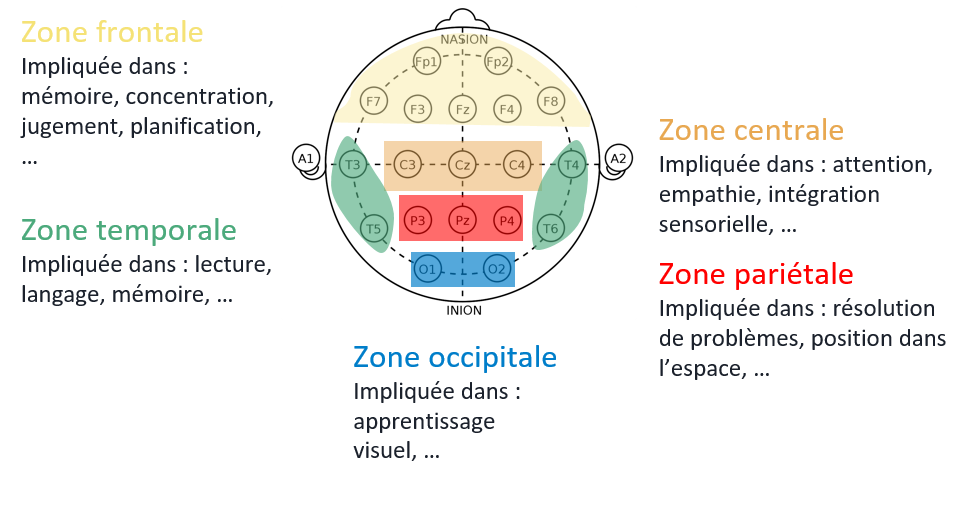
\includegraphics[width=1\linewidth]{figures/chapter-1/introduction_cortical_areas_and_functions} 
  \caption{Schématisation du système \gls{eeg} 10-20. Des exemples de fonctions gérées par les différentes aires cérébrales sont données. }
  \label{Figure:introduction_cortical_areas_and_functions}
\end{figure}

Ainsi, établir un protocole de \gls{nfb} consiste à identifier les rythmes à moduler, s'il faut diminuer ou augmenter la présence de ce neuromarqueur, et l'aire 
du cortex à entrainer en se basant sur la littérature existante.

Les applications du \gls{nfb} peuvent donc être assez diverses, les principales sont décrites ici. 

\subsubsection{Trouble du spectre autistique}

Le trouble du spectre autistique est un trouble neurodeveloppemental qui impacte considérablement les intéractions sociales et qui est toujours présent à 
l'âge adulte. Les \gls{eeg} des enfants autistes présentent des anomalies comparés à ceux des enfants sains, notamment \citep{Coben2010, Kouijzer2010} :
\begin{itemize}
\item une activité dans les hautes fréquence de beta liée à l'anxiété,
\item une forte activité du ratio delta/theta correspondant à un déficit d'attention.
\end{itemize}
Lors de la plupart des entrainements par \gls{nfb} pour traiter le trouble du spectre autistique, il est demandé aux enfants de diminuer à la fois leur ratio 
theta/alpha et d'augmenter la production d'ondes beta \citep{Thompson2010, Othmer2007}. 

\subsubsection{Epilepsie}

La recherche concernant le \gls{nfb} appliqué à l'épilepsie remonte au début de l'utilisation du \gls{nfb} avec \citet{Lubar1976}. Le protocole le plus
couramment utilisé est l'augmentation du \gls{smr} qui mène à une réduction du taux de crises d'épilepsie graves \citep{Hughes2008, Walker2010}.

\subsubsection{Gestion de la douleur}

Le \gls{nfb} a également été étudié dans la diminution de la douleur en visant directement le traitement de la perception de la douleur Le \gls{nfb} a, par
exemple, été utilisé dans le cas de lombalgies chroniques en entrainant les ondes alpha de façon à ce qu'elles soient synchrones sur l'ensemble des aires 
cérébrales \citep{Mayaud2019}.

\subsubsection{Autres applications}

D'autres applications existent comme la diminution de l'anxiété via un protocole de diminution des ondes alpha \citep{Budzynski2009}, le traitement de la dépression
grâce à l'augmentation des ondes alpha et theta tout en diminuant les ondes beta \citep{Hurt2014}. Une application qui fait l'objet de nombreuses recherches
est le \gls{tdah}, décrite plus précisément dans la section suivante.

\subsection{Neurofeedback et \gls{tdah}}

\subsubsection{Définition du \gls{tdah}}

Le \gls{tdah} (\textit{Attention Deficit Hyperactivity Disorder} en anglais) est un trouble psychiatrique qui touche environ 5\% d'enfants en âge d'aller à l'école, 
ce qui représente 2.5 millions d'enfants en Europe \citep{DSM-5}. Ce trouble se caractérise par l'existence de trois groupes de symptômes \citep{HAS} : 
\begin{itemize}
\item le déficit attentionnel : l'enfant est dans l'incapacité de mener une tâche jusqu'au bout, il est distrait, il refuse ou évite les tâches qui demandent
une attention soutenue,
\item l'hyperactivité motrice : l'enfant ne cesse de s'agiter, il ne peut pas rester assis quand les conditions l'exigent, il fait preuve de peu d'organisation,
\item l'impulsivité : l'enfant a du mal à patienter, il a besoin d'agir et a tendance à interrompre les activités d'autrui, notamment en leur coupant la parole.
\end{itemize}
Pour certains enfants, un seul type de symptômes peut être prédominant, alors que d'autres les presentent tous de façon équivalente. Par ailleurs, de récentes 
études ont montré que les différents symptômes évoluent tout au long de la vie du patient \citep{CFDCAP, Epstein2013}.

% evolution du tdah
% tdah chez l'adulte mais non on se concentre sur les enfants 

\subsubsection{Diagnostic du \gls{tdah}}

% dsm4 et dsm5, voir has pour la france
% nebaheath, dire comment le profil eeg des enfants est différent (utiliser article tbr)

\subsubsection{Traitements existants}

% traitement de première intention
% définition thérapies comportementales
% mph (citer des méta-analyses)
% nfb (parler des neuromarqueurs, utiliser l'intro du papier facteurs)

\subsubsection{Efficacité du \gls{nfb}}

% études et méta-analyses
% parler des échelles cliniques, (composantes inattention, hypercativité et totale), dire que plus le score est haut plus on est atteint
% des évaluateurs parents teachers et cliniciens (comme quoi ils sint fiables)


% lien vers la partie suivante : efficacité du nfb est au coeur de cette thèse


En plus des symptômes du \gls{tdah}, le bien être des enfants est impacté : en effet, ces derniers souffrent d'une faible estime d'eux-mêmes et ont de mauvaises notes à l'école

% voir lambez B et al. 2019

%NFB is a self-paced brain neuromodulation technique that
%represents brain activity in real-time using auditory or visual
%modulations, on which learning paradigms, such as operant
%conditioning (37) or voluntary control, can be applied. To deliver
%this intervention, neurophysiological time series are analyzed
%online in order to drive feedback applications such as serious
%games (38). The signal of interest should represent the activity
%of a population of neurons involved in attentional networks,
%which is translated into visual or auditory cues. The sensory
%feedback constitutes the rewardsmechanism, promoting learning
%using, for instance, operant conditioning protocols (39). Operant
%conditioning enables neural plasticity, thus supporting the child
%in the task repetition (40), which is believed to result in longlasting
%neuronal reorganization (41).
%Several NFB protocols have been proposed and investigated
%for decreasing the symptoms of ADHD:
%• protocols based on neural oscillations, using frequency-band
%power training: enhancing SMR (42), reducing theta (29)
%or enhancing beta (43), or a composite protocol such as
%enhancing beta while suppressing theta, also known as the
%Theta Beta Ratio (TBR) protocol (33, 44);
%• protocols based on Slow Cortical Potentials (SCPs) training
%consisting of the regulation of cortical excitation thresholds by
%focusing on activity generated by external cues (45, 46);
%• protocols to enhance Event-Related Potentials (ERPs):
%in particular, the amplitude of the P300 ERP can be
%considered as a specific neurophysiological marker of selective
%attention (47).


% définition du tdah chez l'enfant (symptômes, prévalence)
% diagnostic du tdah (dsm-4 et dsm 5), essor du tdah chez les adultes (10.1001/jamanetworkopen.2019.14344, Chung et al.) mais ici on ne s'intéresse qu'aux enfants
% parler des traitements possibles (methylphenidate, thérapies comportementales et finir sur NFB)
% parler de nebahealht
% neuromarqueurs couramment utilisés (utiliser intro Bussalb2019clinical
% efficacité du nfb à travers les méta-analyses, l'efficacité du nfb est souvent donnée à l'aide d'évaluations sur des échelles cliniques, état de la littérature
% décire les échelles cliniques (composantes inattention, hypercativité et totale)
% les évaluateurs parents et teachers sont reliable selon lambez B et al. 2019, c'est admis de les utiliser comme évaluateurs
% dans les méta-analyses on parle de pblind et de mprox


%Définition TDAH chez l’enfant (parler du dsm-4 et 5) et parler de l’essor de la problématique du TDAH chez l’adulte (10.1001/jamanetworkopen.2019.14344, Chung et al.), parler des études et des méta-analyses
%sham-NFB, parler des échelles cliniques (It is generally accepted that parent and teacher rating scales are reliable and 
%valid components of ADHD assessments (McGough  Barkley, 2004)), définir pblind et mprox, dire que c'est admis de les utiliser comme évaluateurs lambez B et al. 2019
%Parler des traitements possibles (bien définir les cognitives therapy)
%% dire quels sont les neuromarqueurs utilisés et les autre types de nfb

\section{Objectifs de la thèse}

Le \gls{nfb} a fait l'objet de nombreuses études pour déterminer son efficacité dans le cadre du \gls{tdah} chez l'enfant comme souligné précédemment.
Malheureusement, aucun consensus n'a encore été clairement atteint, ainsi le travail effectué au cours de cette thèse a pour but de déterminer les facteurs 
de réussite de l'entraînement par \gls{nfb} pour les enfants \gls{tdah} en se basant sur des données cliniques mais aussi physiologiques. 

Les trois sous objectifs de ce travail, chacun développé dans un chapitre, sont les suivants :
\begin{itemize}
\item étudier l'efficacité du \gls{nfb} chez les enfants \gls{tdah} à l'aide d'une méthode couramment utilisée : la méta-analyse,
\item identifier les paramètres méthodologiques et cliniques influençant la performance de ce traitement,
\item analyser la distribution d'un marqueur de l'attention au sein d'une population d'enfants \gls{tdah} pour mieux cibler
l'entrainement par \gls{nfb}. 
\end{itemize}

\section{Contribution et résumé des chapitres}

Ce manuscrit est divisé en 5 parties, dont les trois centrales (les chapitres \ref{chapitre-2}, \ref{saob} et \ref{chapitre-4}) ont chacune pour but de remplir 
un des objectifs précédemment énoncés.

Avant de chercher à déterminer les facteurs de réussite de l'entrainement par \gls{nfb}, son efficacité sur les enfants \gls{tdah} est évaluée à l'aide 
d'une méthode couramment utilisée \citep{Sonuga-Barke2013, Micoulaud2014, Cortese2016} et présentée dans le chapitre \ref{chapitre-2} : la méta-analyse. 
Les résultats de ce type d'analyse ont un impact important sur la communauté scientifique : \citet{Micoulaud2016} a notamment réagi à la méta-analyse de 
\citet{Cortese2016} en discutant certains points de cette analyse. 

Ainsi, dans ce chapitre la méta-analyse de \citet{Cortese2016} est répliquée en modifiant les points soulignés par \citet{Micoulaud2016}
afin de jauger leur impact sur les conclusions émises dans la méta-analyse. Ensuite, étant donné que de nouvelles études satisfaisant les critères d'inclusion
établis par \citet{Cortese2016} sont disponibles, cette méta-analyse est mise à jour : en plus des 13 études originellement incluses, 3
sont ajoutées, ce qui apporte une plus grande puissance statistique aux résultats. La réplication et la mise à jour sont effectuées, non pas avec les logiciels 
habituellement utilisés tels que Revman \citep{Revman}, mais à l'aide d'un package Python développé pour cette occasion et disponible en ligne afin de favoriser 
la réplication et/ou la mise à jour de ce travail. 

La réplication de la méta-analyse conduisant aux mêmes résultats que \citet{Cortese2016}, les choix discutés par \citet{Micoulaud2016} n'ont pas un impact assez
important pour changer ses conclusions : le \gls{nfb} est jugé efficace par les parents alors que les enseignants, considérés comme \gls{pblind}, ne notent aucune
amélioration significative. Par ailleurs, la mise à jour confirme les résultats qui semblent commencer à se stabiliser pour les évaluations des parents.

Ce chapitre a été l'occasion de mener une revue de littérature des études d'efficacité sur le \gls{nfb} appliqué aux enfants \gls{tdah} 
qui a permis de mettre en évidence la forte hétérogénéité d'un point de vue clinique et méthodologique de ces études. 

Alors que la fiabilité des résultats des méta-analyses souffrent de ces différences qui pourraient, par ailleurs, expliquer l'absence de consensus quant 
à l'efficacité du \gls{nfb} \citep{Alkoby2017}, une analyse en tirant avantage est implémentée : la \gls{saob} décrite dans le chapitre \ref{saob}. 
Les facteurs méthodologiques et/ou cliniques fortement variables entre les études tels que, par exemple, la durée du traitement, le nombre de sessions et le type 
de protocole de \gls{nfb} suivi, sont extraits de 33 études d'efficacité sur le \gls{nfb} appliqué aux enfants \gls{tdah} dans le but de déterminer lesquels 
ont un impact sur l'efficacité du \gls{nfb}. Pour ce faire, trois méthodes multivariées sont utilisées : la \gls{wls}, le \gls{lasso} et le \gls{dt}. 

La \gls{saob} identifie trois facteurs qui semblent avoir un impact sur l'efficacité du \gls{nfb} : tout d'abord, utiliser un matériel d'acquisition de bonne 
qualité conduirait à de meilleurs résultats, ensuite un traitement intensif semblerait préférable, et enfin les évaluations des enseignants seraient plus
sévères quant à l'amélioration du traitement. 

La personnalisation des protocoles de \gls{nfb} est un facteur dont il aurait été intéressant d'étudier l'impact sur l'efficacité du \gls{nfb}.  
Cependant, faute d'un nombre suffisant d'études ayant recours à la personnalisation, ce facteur n'a pas pu être étudié dans la \gls{saob}. C'est pourquoi
la pertinence d'une personnalisation est étudiée dans le chapitre \ref{chapitre-4} grâce à l'analyse de la distribution d'un marqueur de l'attention : le \gls{tbr} pour
lequel de précédentes études ont montré qu'il serait variable au sein de la population \gls{tdah} \citep{Zhang2017, Arns2013, Clarke2001}.

Le \gls{tbr} est extrait de 363 \gls{eeg} d'enfants \gls{tdah} qui vont être partitionnés grâce à trois méthodes : le \gls{bgmm}, le partitionnement
hiérarchique basé sur la distance de Ward et le \gls{dbscan}. Si la distribution est trouvée bimodale par ces trois méthodes, les seuils calculés par chaque méthode,
sont comparés, notamment grâce à une courbe \gls{roc} obtenue sur
les résultats du \gls{bgmm} afin de déterminer celui sur lequel il faudrait se baser pour attribuer le protocole de \gls{nfb}.

Les trois méthodes s'accordent sur le fait que la distribution des \gls{tbr} est bimodale, ce qui indique qu'il existe en effet deux groupes d'enfants
\gls{tdah} : l'un présentant des \gls{tbr} plutôt faibles et l'autre avec des \gls{tbr} élevés. Ainsi, personnaliser le protocole de \gls{nfb} en 
fonction de la valeur de \gls{tbr} semblerait pertinent et après comparaison des seuils \gls{tbr} obtenus, celui de 4.1 apporte le plus d'équilibre entre 
un faible taux de faux positifs et un taux de vrais positifs élevé.  

\section{Liste des publications}

Le travail décrit dans ce manuscrit a donné lieu aux publications avec comité de lecture suivantes :

\begin{description}
\item \citet{Bussalb2019tbr} : A. Bussalb, S. Collin, Q. Barthélemy, D. Ojeda, E. Acquaviva, S. Bioulac, H. Blasco-Fontecilla,
D. Brandeis, R. Delorme, D. P. Ouakil, T. Ros, and L. Mayaud. Is there a cluster of high
theta-beta ratio patients in attention deficit hyperactivity disorder ? \textit{Clinical Neurophysiology}, 2019a.
\item \citet{Bussalb2019clinical} : A. Bussalb, M. Congedo, Q. Barthélemy, D. Ojeda, E. Acquaviva, R. Delorme,
and L. Mayaud. Clinical and experimental factors influencing the efficacy of
neurofeedback in ADHD: a meta-analysis. \textit{Frontiers in psychiatry}, 10 :35, 2019b.
\end{description}

Une partie des travaux de \citet{Bussalb2019clinical} ont fait l'objet d'une communication orale :

\noindent A. Bussalb, M. Congedo, R. Delorme, E. Acquaviva, Q. Barthelemy, D. Ojeda, J.A. Micoulaud-Franchi, L. Mayaud. Neurofeedback 
appliqué aux enfants TDAH : quels facteurs influencent son efficacité ? 6ème Congrès de la SOFTAL, mai 2018. 


